\documentclass[tikz,convert={density=150,size=600,outext=.png}]{standalone}
\usetikzlibrary{shapes, calc, arrows, fit, positioning, decorations, patterns, decorations.pathreplacing, chains, snakes}

\begin{document}
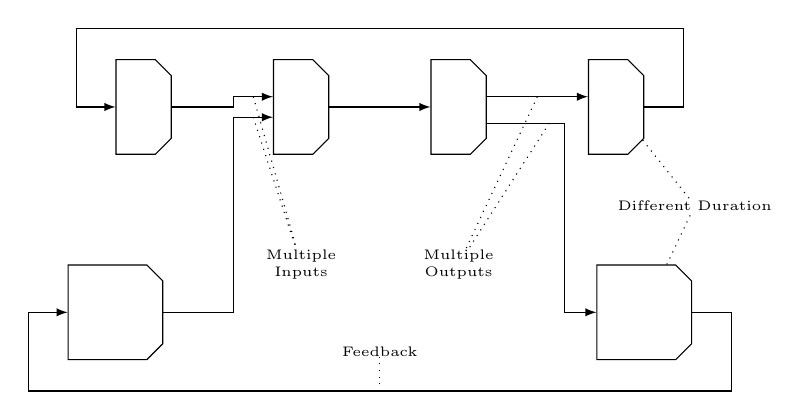
\begin{tikzpicture}[>=latex, text width=0.5cm, text badly centered, inner ysep=0.5cm, inner xsep=0cm, node distance=2cm, font=\tiny]
\node[draw, chamfered rectangle, chamfered rectangle corners={north east, south east}] (u11) {};
\node[draw, chamfered rectangle, chamfered rectangle corners={north east, south east}, right of=u11] (u12) {};
\node[draw, chamfered rectangle, chamfered rectangle corners={north east, south east}, right of=u12] (u13) {};
\node[draw, chamfered rectangle, chamfered rectangle corners={north east, south east}, right of=u13] (u14) {};
\node[text width=1cm, draw, chamfered rectangle, chamfered rectangle corners={north east, south east}, below=of u11.west] (u21) {};
\node[text width=1cm, draw, chamfered rectangle, chamfered rectangle corners={north east, south east}, below =of u14.east] (u22) {};

\draw[->] (u11.east) -| ([xshift=-0.5cm] u12.160) -- (u12.160) coordinate[pos=0.5] (e1);
\draw[->] (u12.east) -- (u13.west);
\draw[->] (u13.30) |- (u14.160) coordinate[pos=0.75] (e3);;
\draw[->] (u13.-30) -|  coordinate[pos=0.4] (e4) ([xshift=-0.4cm] u22.west) -- (u22.west);
\draw[->] (u21.east) -|  ([xshift=-0.5cm] u12.200) -- (u12.200) coordinate[pos=0.5] (e2);
\draw[->] (u22.east) -|  ([xshift=0.5cm, yshift=-1cm] u22.east) -| ([xshift=-0.5cm] u21.west) coordinate[pos=0.25] (e5) -- (u21.west);
\draw[->] (u14.east) -|  ([xshift=0.5cm, yshift=1cm] u14.east) -| ([xshift=-0.5cm] u11.west) -- (u11.west);

\node[below of=u12, inner sep=0cm, text width=1cm] (multi-inputs) {Multiple Inputs};
\node[below of=u13, inner sep=0cm, text width=1cm] (multi-outputs) {Multiple Outputs};
\node[above of=e5, node distance = 0.5cm,  inner sep=0cm, text width=2cm] (back-edges) {Feedback};
\node[below of=u14, node distance = 1.25cm,  inner sep=0cm, text width=2cm, xshift=1cm] (delay) {Different Duration};

\draw[dotted] (e1) -- (multi-inputs);
\draw[dotted] (e2) -- (multi-inputs);

\draw[dotted] (e3) -- (multi-outputs);
\draw[dotted] (e4) -- (multi-outputs);

\draw[dotted] (e5) -- (back-edges);

\draw[dotted] (u14) -- (delay);
\draw[dotted] (u22) -- (delay);
\end{tikzpicture}
\end{document}
